% Section content template for individual Educative lessons
% This file contains the actual content for a specific section
% Generated from Educative API section content

% Section: Activity Diagram for the Parking Lot
% Section ID: 5488447435571200
% Section Slug: activity-diagram-for-the-parking-lot
% Generated: 2025-12-11T13:40:36.558112

An activity diagram is a great way to visualize the flow of messages from one activity to another in the system. There can be different activity diagrams that we can create for our parking lot system. For this lesson, we will create activity diagrams for the following two activities:

\begin{itemize}
\item
\protect\phantomsection\label{RfPyJ0ULta3W-nF0-Gk5j}
The vehicle enters the parking lot.
\item
\protect\phantomsection\label{CuQ7mq3zk-n22j4-50gdP}
\textbf{Activity challenge:} Customer pays the parking ticket.
\end{itemize}

\subsection{Vehicle entering the parking lot}\label{Xz3VksdTTnj4oxHLC94rY}
\\
The following are the states and actions that will be involved in this activity diagram.

\subsubsection{States}\label{d47qDFSzxJJdTDK7Dm7kd}
\\
\textbf{Initial state:} The customer enters the parking lot.
\\
\textbf{Final state:} There are two final states present in this activity diagram, shown below:

\begin{itemize}
\item
\protect\phantomsection\label{U0DnNrey23SHusPFeXlli}
The customer receives the parking ticket through the system.
\item
\protect\phantomsection\label{PJQn4h98mDi6o5ZcbhIf6}
There is no vacant parking slot, so the customer is denied access to the parking lot.
\end{itemize}

\subsubsection{Actions}\label{O0z4gIIbFtDE1NdhXE_o5}
\\
The customer arrives at the parking lot entrance and selects their vehicle type. They are assigned their dedicated parking spot according to their select vehicle type. The parking lot then informs us about the availability of that parking spot and allows access accordingly.
\\
The activity diagram of a vehicle entering a parking lot is given below based on the order above.
\begin{quote}
\textbf{Note:} Here, we assume that only vehicles displaying a valid disability permit can park in the designated accessible spot.
\end{quote}

\begin{figure}[htbp]
 \centering
 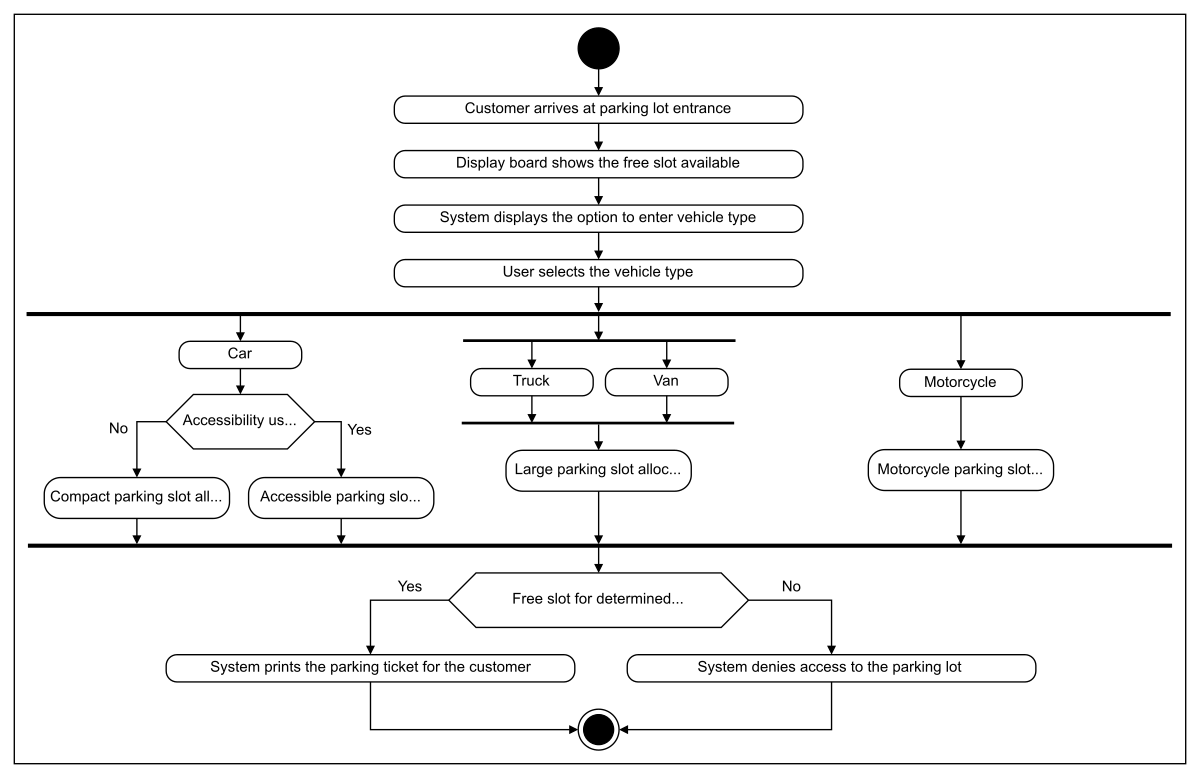
\includegraphics[width=0.5\textwidth]{Images/chapter_7/section_5488447435571200/4696554780622848.png}
 \caption{The activity diagram for the vehicle entering a parking lot}
\end{figure}

\subsection{Activity challenge: The customer pays the parking ticket}\label{qQ8UiLDWEEf6Cnibbq9TJ-1}
\\
You will help us create an activity diagram of a customer paying a parking ticket at the exit panel.
\\
The skeleton of the activity diagram below represents that the customer has a valid parking ticket available.

\begin{figure}[htbp]
 \centering
 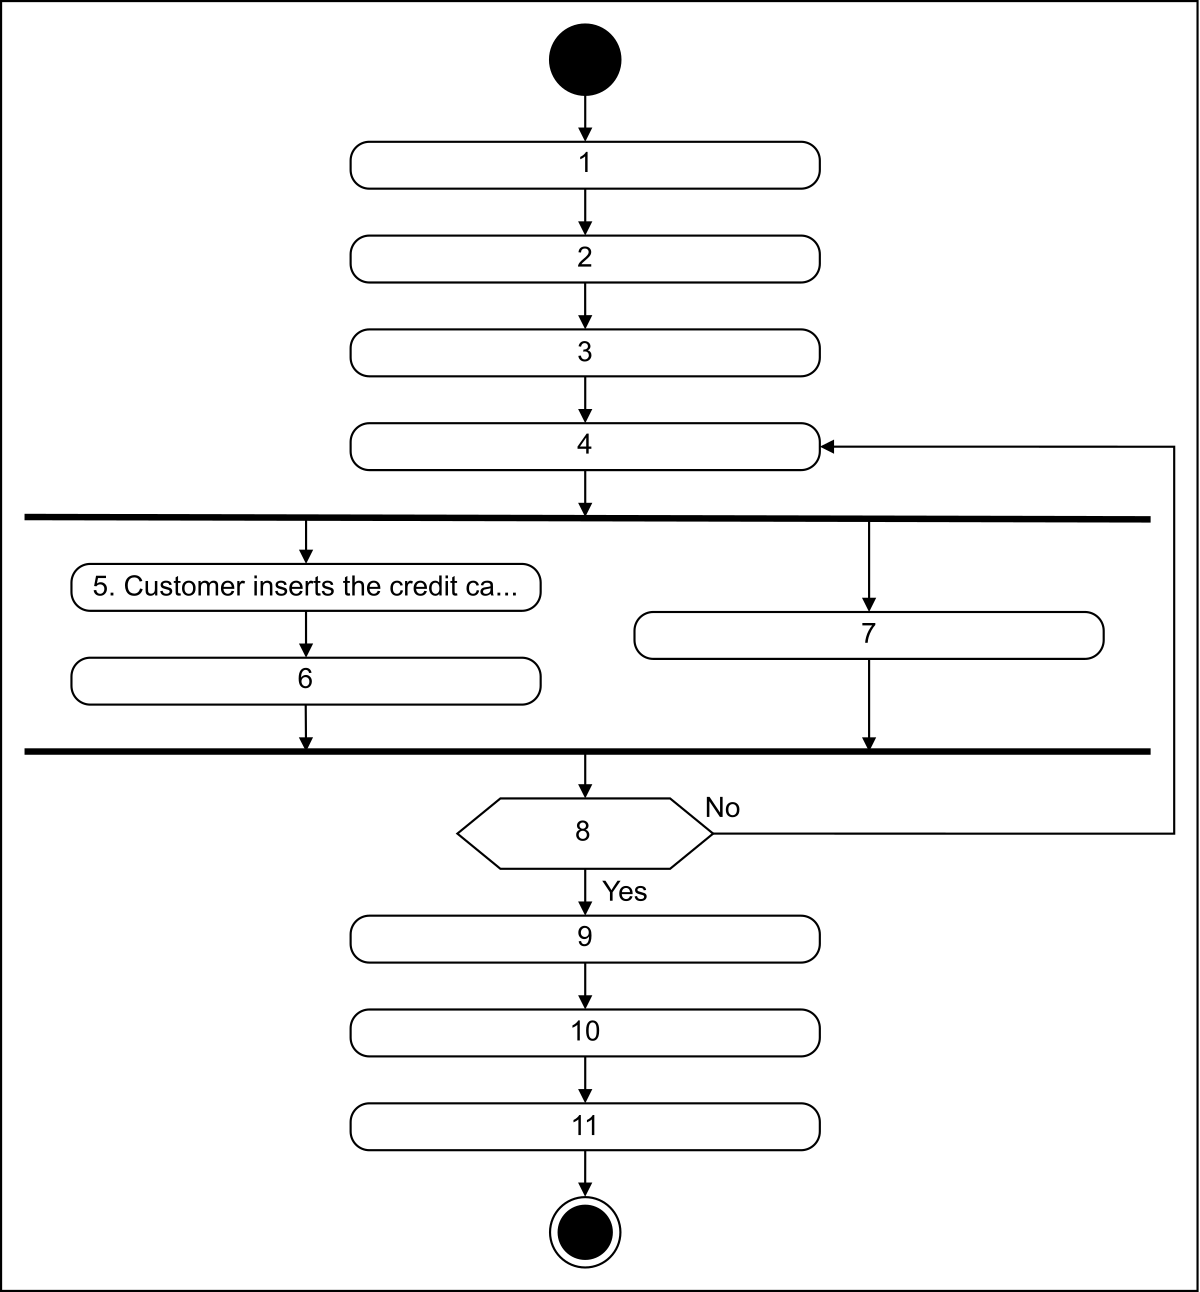
\includegraphics[width=0.5\textwidth]{Images/chapter_7/section_5488447435571200/6620874053779456.png}
 \caption{The activity diagram for the vehicle entering a parking lot}
\end{figure}

Notice that the actions in the diagram above are numbered from 1 to 11. The slots shown below represent the activities, and the arrows represent the flow from one activity to the other. Can you rearrange the slots below in the correct order they should appear in the activity diagram above?
\\
Based on the description above, can you fill in the missing slots with the correct order of actions in the activity diagram?
\begin{quote}
\textbf{Note:} If you're stuck, click the ``Show Solution'' button.
\end{quote}

Alternatively, you can also click the ``Show complete diagram'' button below to see the complete sequence diagram.

We've examined some of our parking lot system's activity diagrams. In the next lesson, we will present the code for our designed classes in some of the most popular languages.

% End of section content